\section{Works Done}
\label{sec:worksDone}


\subsection{Electronics}

In this week, we have tested the batteries and regulators.
Batteries are 3.7 li-ion batteries, and regulators are 5V, 1.2 mA DC to DC boost converters. Batteries work properly, however we have some issues with the converters. The output voltage of the regulator varies with the variation at the input voltage. For example, when 3.3V is given to the converter, output voltage is 5.25V. When 3.9V is given, output voltage is 5.35V. These small differences at the outputs of the regulators may affect the operation of microprocessor and motor. This problem might be solved by adding capacitors and resistors at the output of the regulator. However, the added components will affect the currents which are flowing through the microprocessor and motor. This will affect the performance of our circuit. We are trying to find better solutions to stabilize the voltage output of the regulator.

We bought a weight sensor which can sense up to 50 kilograms and a driver for the sensor. Weight information will be used for feeding regimes and classifications of cats. Test of the sensor will be done in the following week. The images for the sensor and driver are shown in \ref{fig:loadsensor} and \ref{fig:loadsensordriver}.The load sensor gives analog outputs. In order to obtain digital outputs, we bough the sensor driver which contains a 24 bit analog to digital converter. HX711 driver operates properly in the range 2.6 and 5.5V, and its maximum current is 1.5mA [1]. This driver will be supplied from the microprocessor.

\begin{figure}[h]
     \centering
     \begin{subfigure}[b]{0.49\linewidth}
     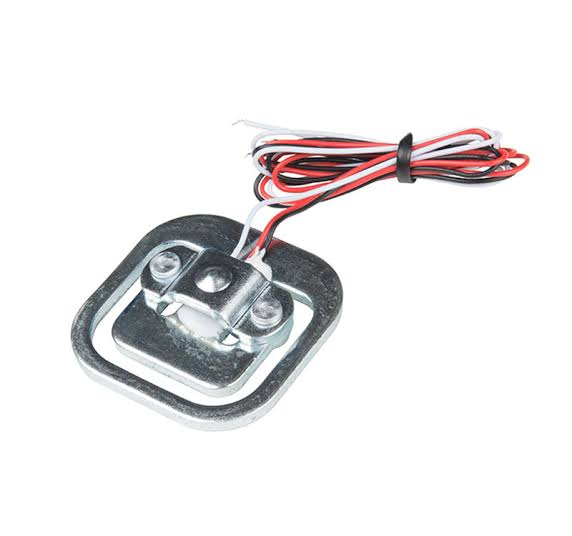
\includegraphics[width=\linewidth]{content/loadsensor.jpeg}
     \caption{Weight sensor}
     \label{fig:loadsensor}
     \end{subfigure}
     \begin{subfigure}[b]{0.49\linewidth}
     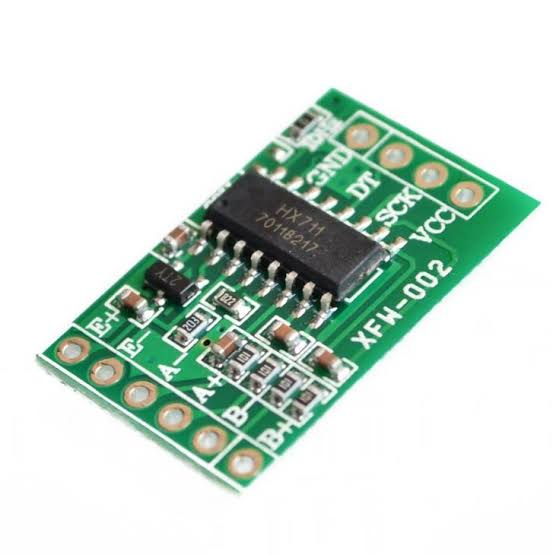
\includegraphics[width=\linewidth]{content/loadsensordriver.jpeg}
     \caption {Weight sensor driver}
     \label{fig:loadsensordriver}
     \end{subfigure}
     \caption{Weight sensor and driver}
     \label{fig:sensorsWeight1}
\end{figure}

\begin{figure}[h]
     \centering
     \begin{subfigure}[b]{0.49\linewidth}
     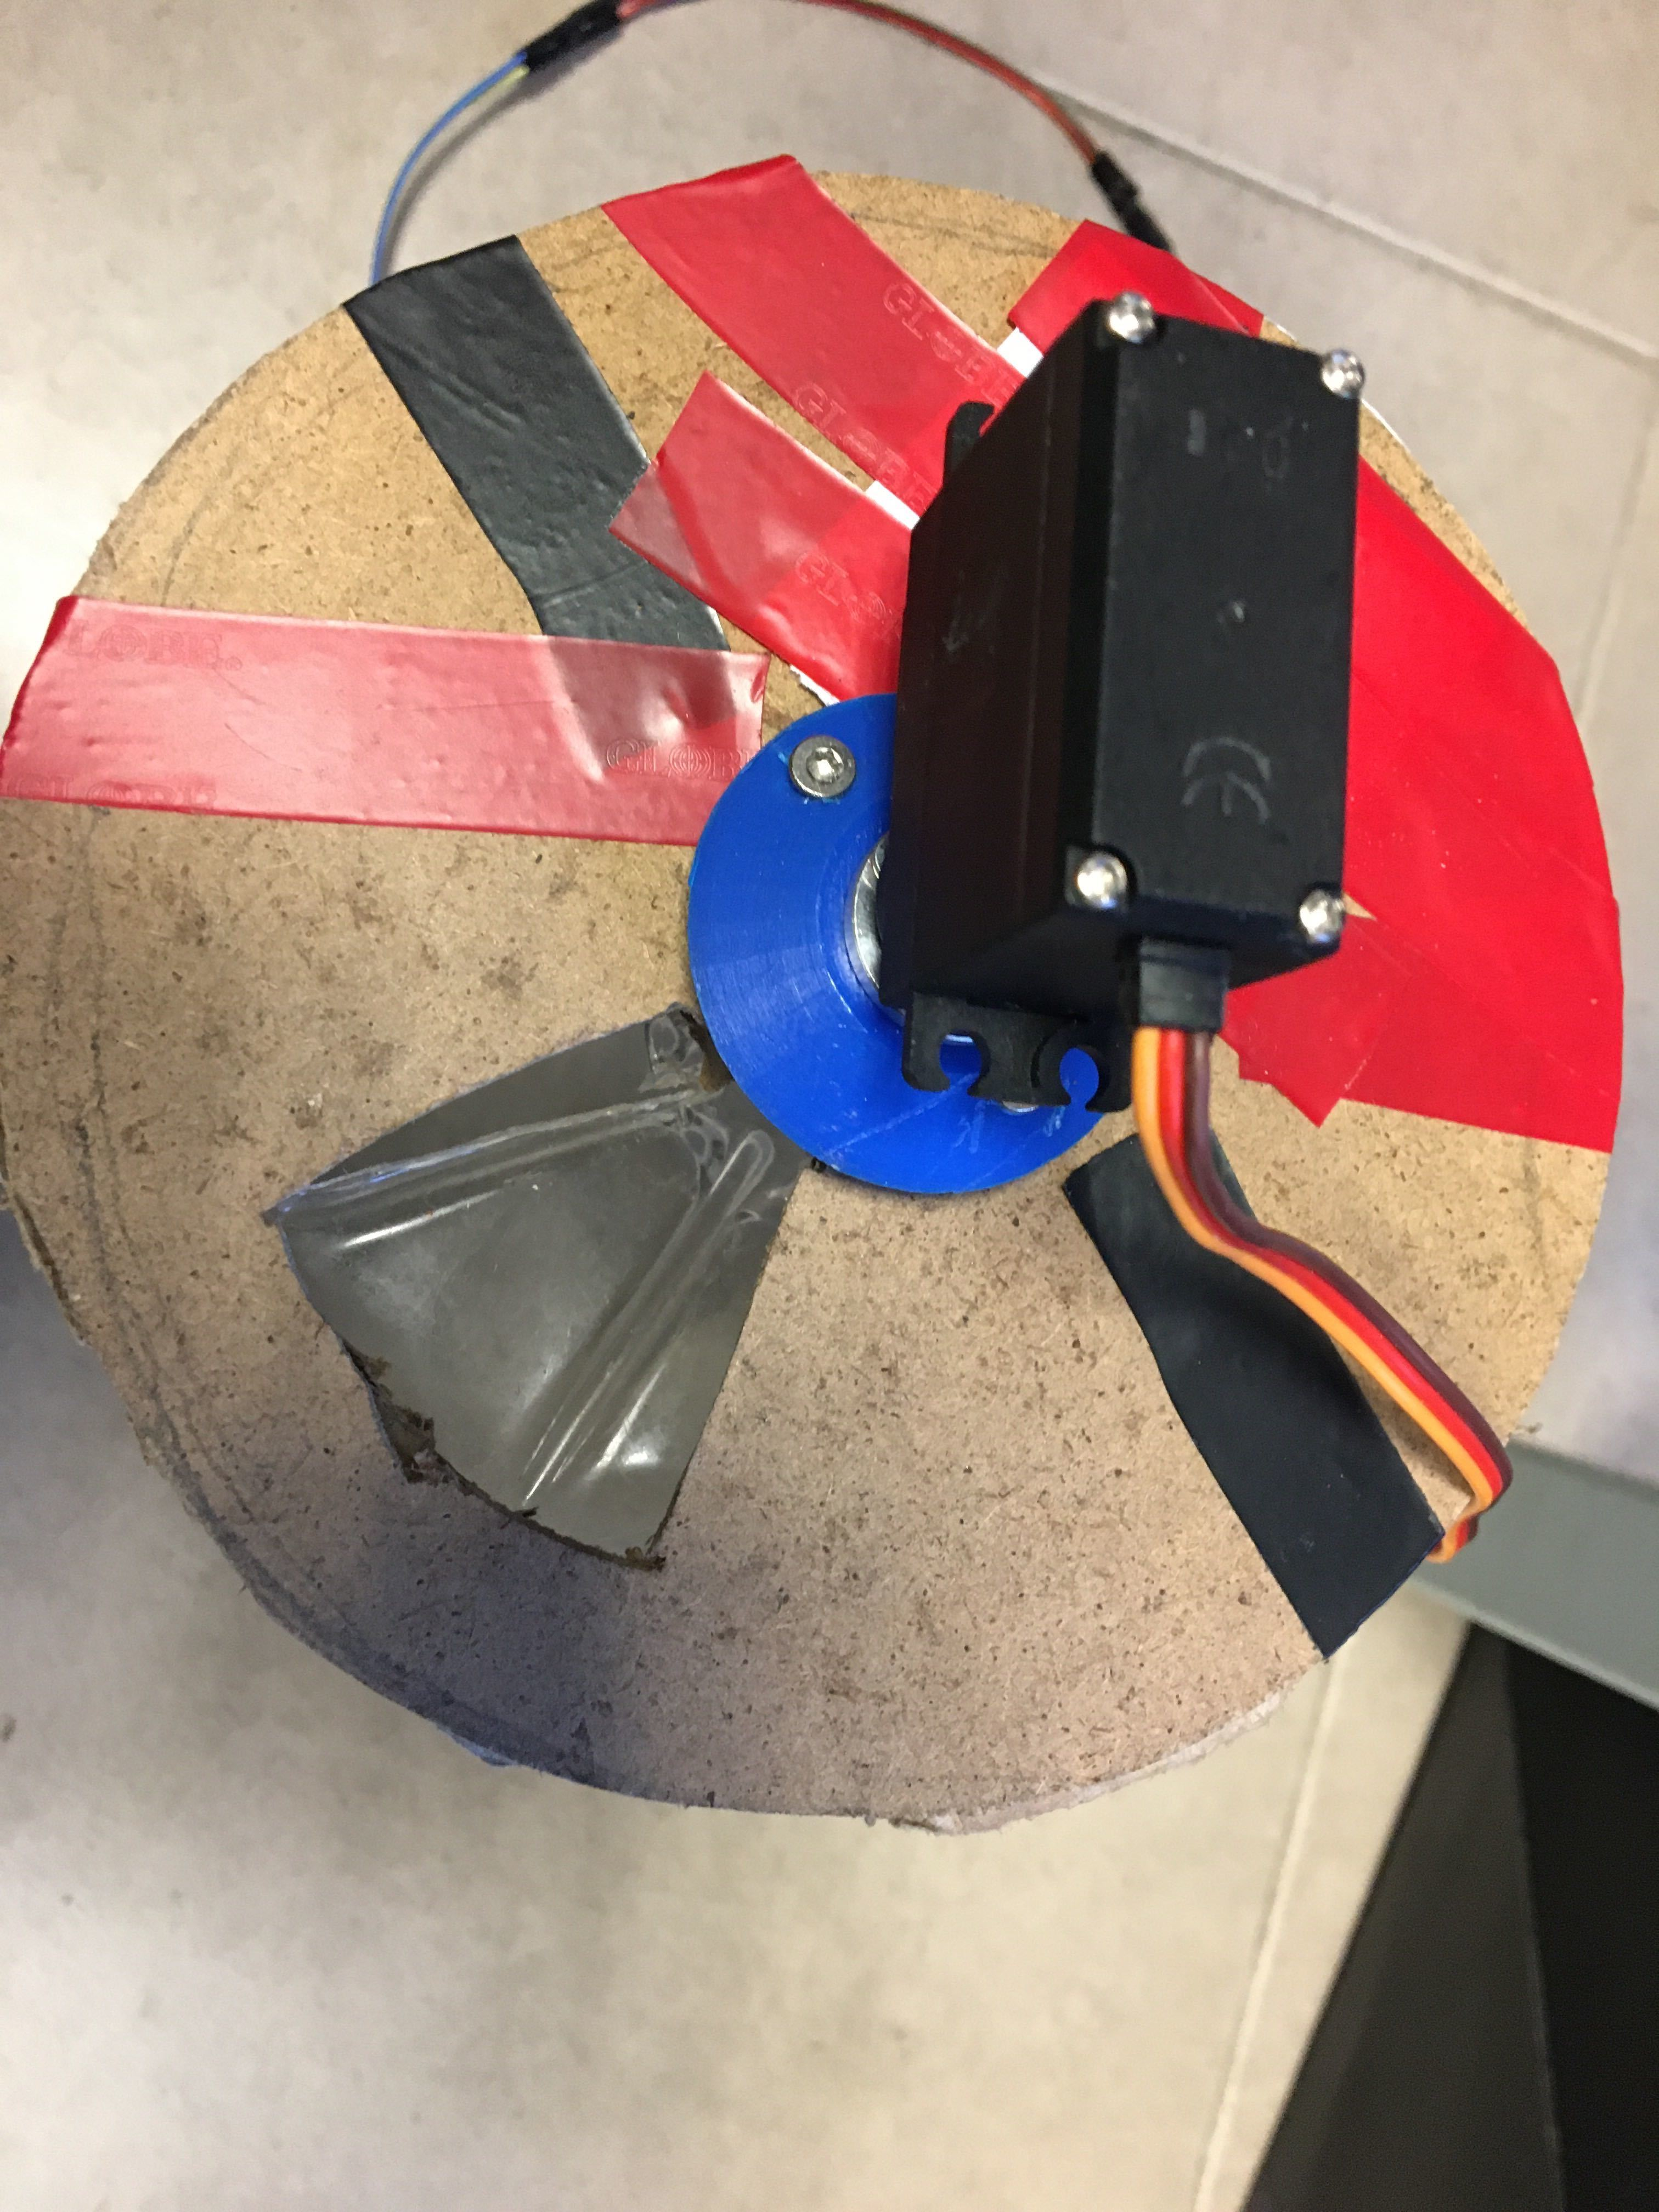
\includegraphics[width=\linewidth]{content/kapak.jpg}
     \caption{Gate Design}
     \label{fig:gate}
     \end{subfigure}
     \begin{subfigure}[b]{0.49\linewidth}
     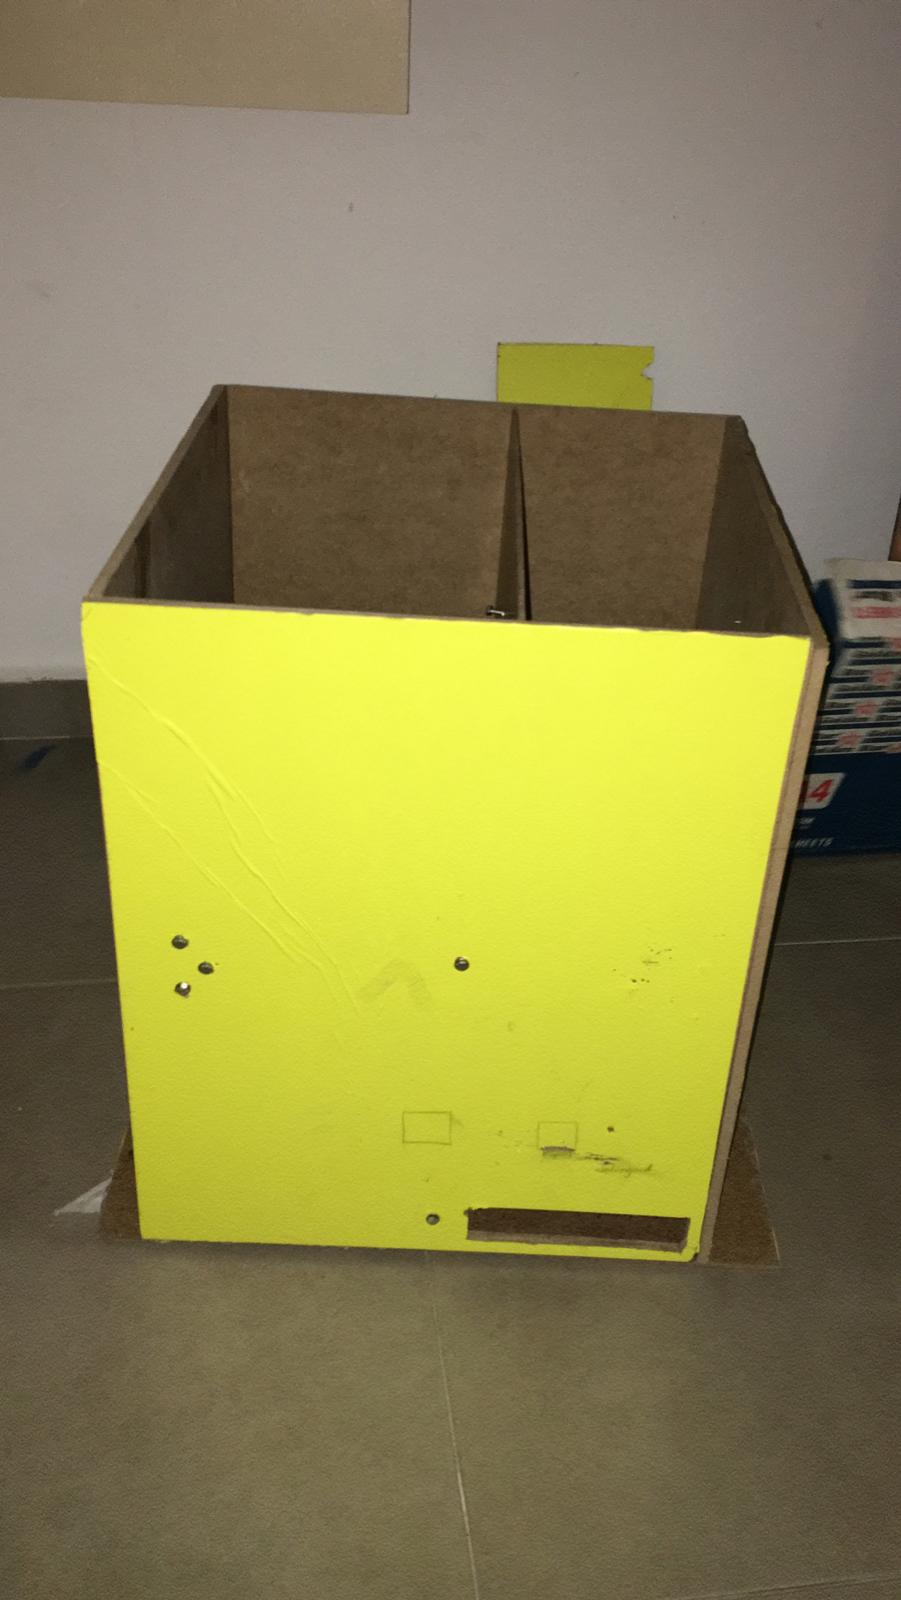
\includegraphics[width=\linewidth]{content/Kutu.jpeg}
     \caption {Body Design}
     \label{fig:body}
     \end{subfigure}
     \caption{Gate and Body}
     \label{fig:bodyandgate}
\end{figure}


\subsection{Mechanics}
This week the outer design of the box is done. Its picture can be seen below. 




In order to solve the wobbling problem, an apparatus was drawn using Siemens NX software and it is planned to be printed on next week. 

Mg996R Servo motor has come and first test are conducted using it. It was observed that, the torque will be more than enough and its balance is good while lifting the food. 

It was decided that, in order to control the amount of food flow, we can use a cylinder shaped device that it can keep the food in its receptacle and when cat has come, and it can empty its receptacle by rotating through the vacancy. When two empty sides are coincided the food will be poured into the reservoir that we have provided for cat to eat. By repeating this process we can control the amount of food given. The figure for this cylinder can be seen below. 

\begin{figure}[h]
     \centering
     \begin{subfigure}[b]{0.49\linewidth}
     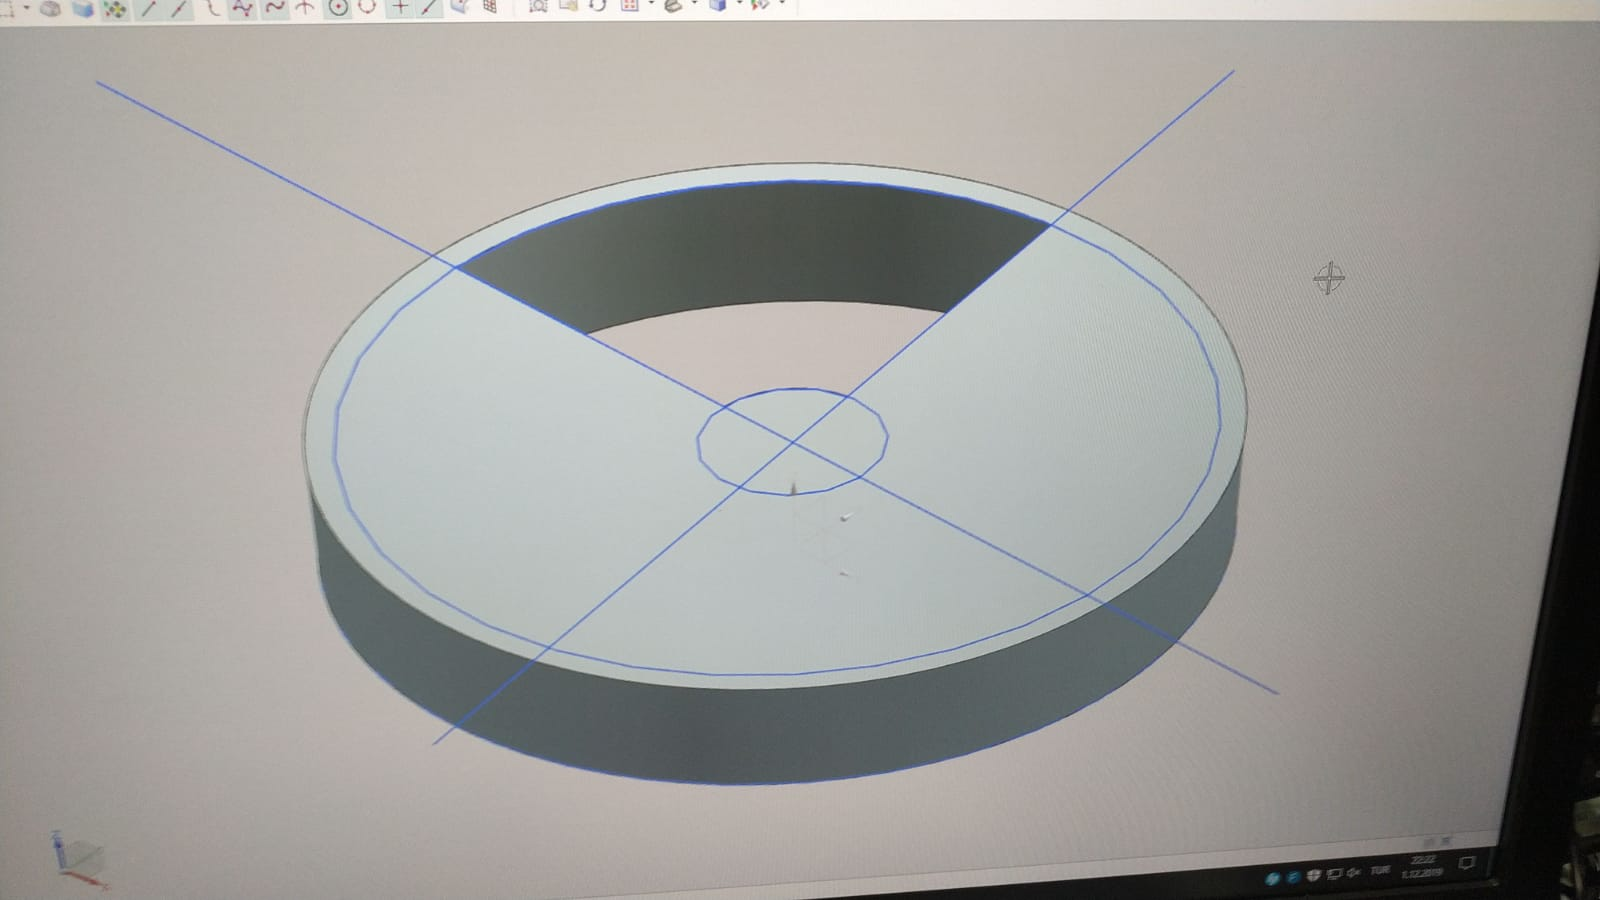
\includegraphics[width=\linewidth]{content/cylinder.jpeg}
     \caption{Design of the Gate}
     \label{fig:cylinder}
     \end{subfigure}
     \begin{subfigure}[b]{0.49\linewidth}
     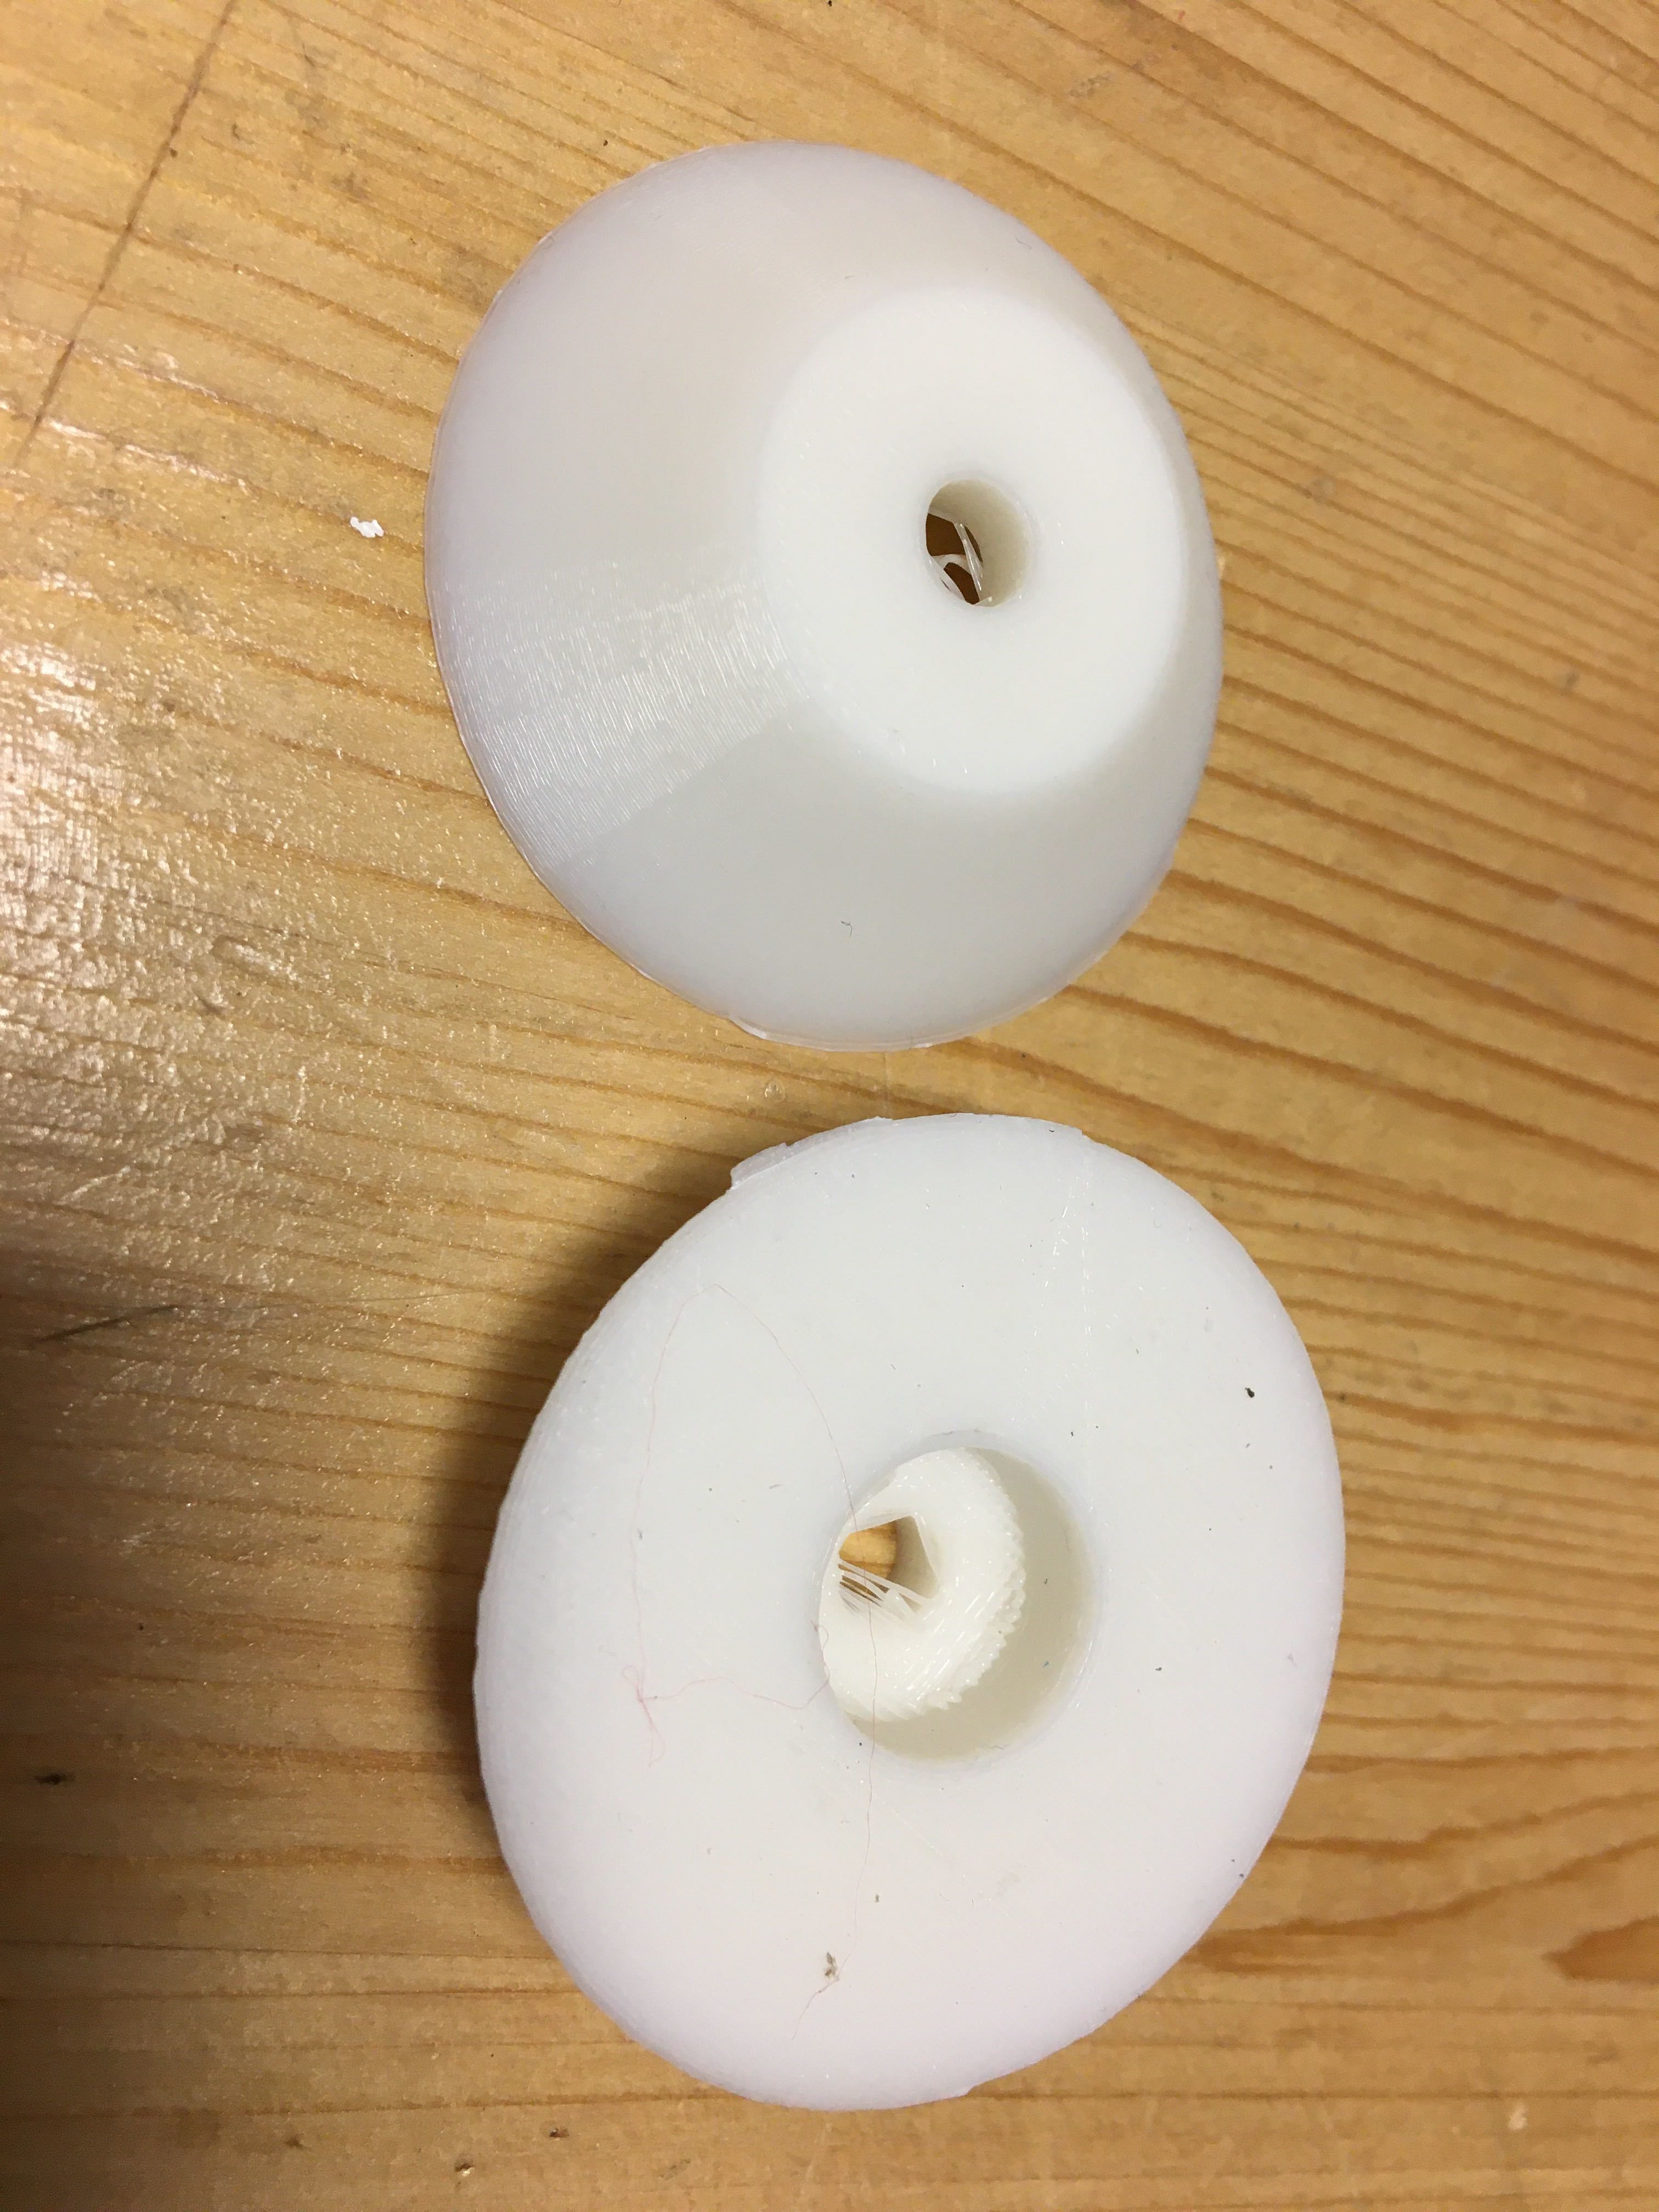
\includegraphics[width=\linewidth]{content/3dprint.jpg}
     \caption {3D Print}
     \label{fig:3dprint}
     \end{subfigure}
     \caption{3D Print and Design of the Gate}
     \label{fig:cylinder3d}
\end{figure}

Food will flow through its empty side and it will be preserved there until a cat arrives. When it arrives, the apparatus rotates and food flows through vacancy.

\subsection{Computer Vision}

Fine tuning will be performed to improve the adaptation of the classifier to the camera's captures. For that, pictures of dogs and cats are collected. Also, SIFT is being implemented to identify cat features.